\documentclass{standalone}

%maths
\usepackage{mathtools}
\usepackage{amsmath}
\usepackage{amssymb}
\usepackage{amsfonts}

%tikzpicture
\usepackage{tikz}
\usepackage{scalerel}
\usepackage{pict2e}
\usepackage{tkz-euclide}
\usetikzlibrary{calc}
\usetikzlibrary{patterns,arrows.meta}
\usetikzlibrary{shadows}
\usetikzlibrary{external}

%pgfplots
\usepackage{pgfplots}
\pgfplotsset{compat=newest}
\usepgfplotslibrary{statistics}
\usepgfplotslibrary{fillbetween}

%colours
\usepackage{xcolor}

\begin{document}

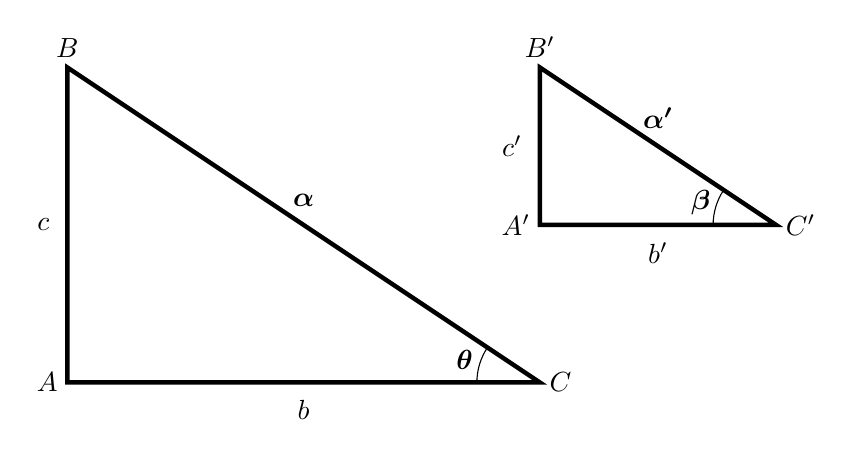
\begin{tikzpicture}
% \draw[lightgray] (-1,-1) grid (10,5);

\coordinate[label=left:$A$] (A) at (0,0);
\coordinate[label=above:$B$] (B) at (0,4);
\coordinate[label=right:$C$] (C) at (6,0);

\draw[ultra thick] (A)--(B)--(C)--cycle;

\tkzLabelSegment[below=3pt](A,C){$b$}
\tkzLabelSegment[left=3pt](A,B){$c$}
\tkzLabelSegment[above=3pt](B,C){$\boldsymbol{\alpha}$}

% \tkzMarkAngle[size=0.8, mark=||](B,C,A)
\tkzMarkAngle[size=0.8](B,C,A)
\tkzLabelAngle[pos=1.0](B,C,A){$\boldsymbol{\theta}$}

\coordinate[label=left:$A'$](A')at(6,2);
\coordinate[label=above:$B'$](B')at(6,4);
\coordinate[label=right:$C'$](C')at(9,2);

\draw[ultra thick] (A')--(B')--(C')--cycle;

\tkzLabelSegment[below=3pt](A',C'){$b'$}
\tkzLabelSegment[left=3pt](A',B'){$c'$}
\tkzLabelSegment[above=3pt](B',C'){$\boldsymbol{\alpha'}$}

\tkzMarkAngle[size=0.8](B',C',A')
\tkzLabelAngle[pos=1.0](B',C',A'){$\boldsymbol{\beta}$}

\end{tikzpicture}

\end{document}


